\documentclass{amsart}
\usepackage{amsmath}
\usepackage{amssymb}
\usepackage{graphicx}
\usepackage{geometry}
\geometry{a4paper}

\title{Homework 1}
\author{Jason Medcoff}
\date{}

\begin{document}
	\maketitle
	
	\noindent{\textbf{Question 1.}}
	\begin{enumerate}
		\item The process is interrupted
		\item The process is scheduled to run
		\item N/A
		\item The process finishes an I/O or device operation
		\item N/A
		\item The process requests an I/O or device operation
	\end{enumerate}
	
	$\newline$
	\noindent{\textbf{Question 2.}}
	\begin{enumerate}
		\item Ready
		\item Running
		\item User
		\item Blocked % double check this
		\item Kernel
		
		\item Yes
		\item Ready
		\item Blocked
		\item Ready
		\item Running, User
		
		\item Running, Ready
		\item Ready, Running
		\item Kernel
		\item Ready
		\item User
		
		\item Ready
	\end{enumerate}
	
	$\newline$
	\noindent{\textbf{Question 3.}}
	Consider a situation where a user is listening to music on a computer, phone, or media player. The entire song need not be loaded into memory for the whole listening duration; since the audio plays back at a constant rate of 44.1 thousand samples per second, we can chunk playback every several seconds, and we only need to load a single chunk at a time. Therefore, while listening to a song, several I/O operations need to take place. This process is called buffering, and every chunk is loaded into a fixed size buffer in memory.
	
	The following state transitions are observed:
	\begin{itemize}
		\item New to Ready: the music player is opened, awaiting song selection
		\item Ready to Running: a song is selected to play (first time), or the next chunk is being played (all other occurrences)
		\item Running to Ready: the song is paused or playback is otherwise interrupted
		\item Running to Waiting: the next chunk of audio must be loaded from disk
		\item Waiting to Ready: the next chunk has successfully been loaded into the buffer
		\item Running to Terminated: Song playback is finished and the music player is closed
	\end{itemize}

	The state transitions are summarized in graphical form in figure \ref{statediagram}. We can see that ``Running" represents playback via the sound card, ``Ready" indicates that audio is on standby, and ``Waiting" shows that disk streaming is being performed.

	
	\begin{figure}\caption{Process State Diagram}\label{statediagram}
		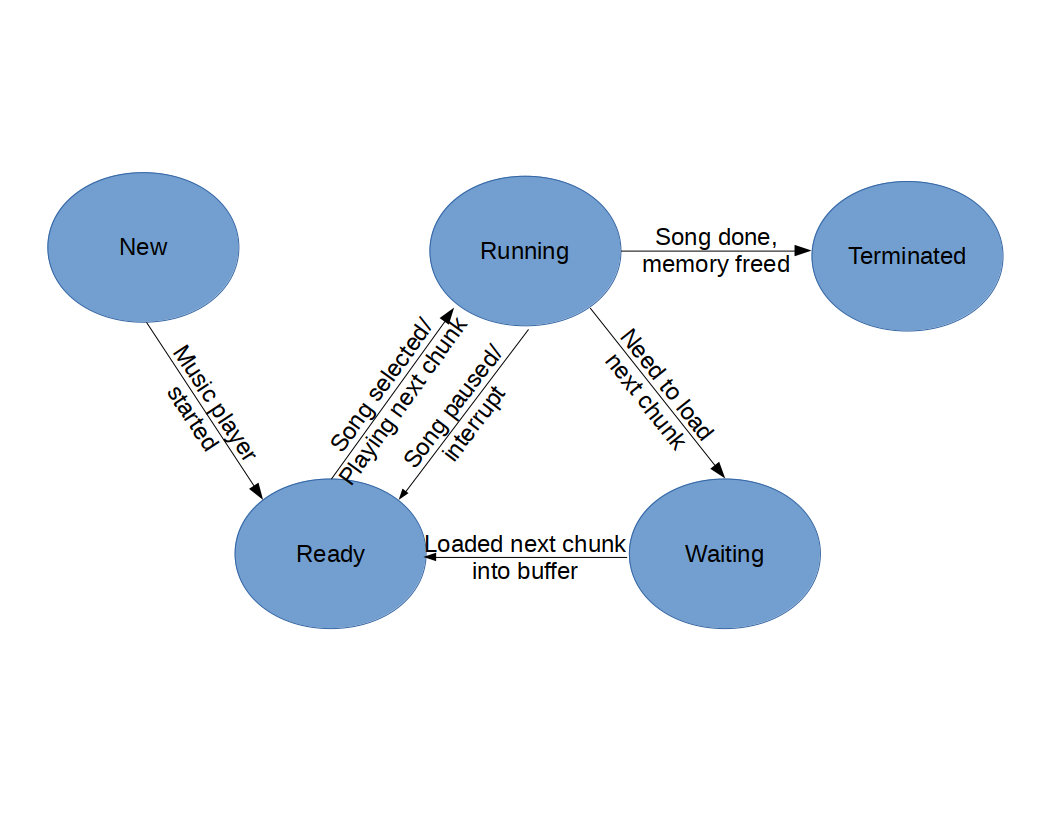
\includegraphics[scale=0.5]{diagram.png}
	\end{figure}
	
	
	
	
	
	
	
	
	
\end{document}